\documentclass[11pt]{article}

% ------------------------------------------------------------------
% Encoding, fonts, language
% ------------------------------------------------------------------
\usepackage[T1]{fontenc}
\usepackage[utf8]{inputenc}
\usepackage{lmodern}
\usepackage{microtype}

% ------------------------------------------------------------------
% Page geometry
% ------------------------------------------------------------------
\usepackage[margin=1in]{geometry}
\raggedbottom

% ------------------------------------------------------------------
% Math
% ------------------------------------------------------------------
\usepackage{mathtools}          % superset of amsmath
\usepackage{amssymb}
\usepackage{amsthm}

\theoremstyle{plain}
\newtheorem{proposition}{Proposition}
\newtheorem{lemma}[proposition]{Lemma}
\theoremstyle{definition}
\newtheorem{definition}{Definition}
\theoremstyle{remark}
\newtheorem*{remark}{Remark}

% ------------------------------------------------------------------
% Tables and figures
% ------------------------------------------------------------------
\usepackage{graphicx}
\usepackage{booktabs}
\usepackage{tabularx}
\usepackage{array}
\usepackage[table]{xcolor}
\usepackage{ragged2e}
\usepackage[font=small,labelfont=bf,labelsep=period]{caption}
\usepackage{tikz}
\usetikzlibrary{positioning,arrows.meta,fit}

% ------------------------------------------------------------------
% Lists
% ------------------------------------------------------------------
\usepackage{enumitem}
\setlist{nosep,leftmargin=*}

% ------------------------------------------------------------------
% Cross-references and URLs
% ------------------------------------------------------------------
\usepackage{hyperref}
\usepackage{xurl}
\usepackage{fancyhdr}

\hypersetup{
  colorlinks  = true,
  linkcolor   = black,
  citecolor   = black,
  urlcolor    = {blue!70!black}
}

% ------------------------------------------------------------------
% Custom column types
% ------------------------------------------------------------------
\newcolumntype{L}[1]{>{\RaggedRight\arraybackslash}p{#1}}
\newcolumntype{Y}{>{\RaggedRight\arraybackslash}X}

% ------------------------------------------------------------------
% Float placement tuning
% ------------------------------------------------------------------
\setcounter{topnumber}{3}
\setcounter{bottomnumber}{2}
\setcounter{totalnumber}{5}
\renewcommand{\topfraction}{0.85}
\renewcommand{\bottomfraction}{0.7}
\renewcommand{\textfraction}{0.12}
\renewcommand{\floatpagefraction}{0.75}

% ------------------------------------------------------------------
% Paragraph and line-breaking
% ------------------------------------------------------------------
\setlength{\emergencystretch}{2em}
\widowpenalty=10000
\clubpenalty=10000

\newcommand{\orcidauthorA}{0009-0009-7659-5964}
\newcommand{\orcidicon}{\includegraphics[width=0.32cm]{../../sixbirds-mathematics/tex/math_instantiation/Definitions/logo-orcid.pdf}}
\newcommand{\orcidA}{\href{https://orcid.org/\orcidauthorA}{\orcidicon}}

\fancypagestyle{firstpage}{%
  \fancyhf{}
  \fancyfoot[C]{\scriptsize Automorph Inc., Wilmington, DE, USA ioannis@automorph.io Zenodo DOI: \href{https://doi.org/10.5281/zenodo.23118249}{10.5281/zenodo.23118249} \textcopyright\ 2026 CC-BY 4.0}
  \renewcommand{\headrulewidth}{0pt}
  \renewcommand{\footrulewidth}{0pt}
}

% ==================================================================
\begin{document}

\title{To Classify a Stone with Six Birds:\\[4pt]
Primitive Activation and Observable Separation\\[2pt]
of Layer-Birth Classes}
\author{Ioannis Tsiokos\;\orcidA{}}
\date{Version 2: October 3, 2026\\[2pt]
\small Version 1: March 16, 2026}

\maketitle
\thispagestyle{firstpage}

\begin{abstract}
\noindent
A \emph{layer birth} is the point at which a coarse-grained description of a stochastic system starts to behave like a theory in its own right, with stable macrostates that it reproduces under its own dynamics. This paper asks whether such births come in different kinds, and how one would tell them apart by measurement. Using the primitive vocabulary of the Six-Birds framework, we classify a birth by three switches: whether \emph{packaging} ($P5$) produces stable objects, whether a genuinely \emph{directed circulation} ($P6_{\mathrm{drive}}$) is present at birth, and whether \emph{staging} structure ($P4$) moves the birth when the observation timescale changes. Requiring packaging leaves four classes: Class-I (packaging only), Class-II (with drive), Class-III (with staging), and Class-IV (with both). We define each switch through finite-state observables---closure error and objecthood for packaging, stationary time-reversal divergence (affinity) for drive, and the timescale shift of both structural boundaries for staging---and give one explicit kernel family for each class. All four representatives are classified correctly on their declared finite grids, and the classification is certified in exact rational arithmetic at ten (class, size) points, including Class-III and Class-IV at sizes 16 to 128. For the undriven Class-III family, a strong-lumpability argument shows that its operational signature is the same at every admissible size. On a common map at size 64, the four classes occupy distinct regions. The Class-I/Class-II contrast is the most robust result: it rests on an exactly zero versus a clearly positive affinity, and it is protected by no-fake-arrow controls. The staging classes are confirmed only for the manual coarse-graining lens and lose their staging label under the two automatic lenses we tried. Capacity/depth proxies and three kernels built from upstream compiled features add context but do not classify. The results are finite and operational: we make no universality-exponent claim, no claim of robustness to arbitrary lenses, and no claim that the upstream system realizes all four classes.
\end{abstract}

\bigskip


\section{Introduction}
\label{sec:introduction}

Coarse-graining usually loses information. Occasionally, though, a coarse description becomes self-sufficient: its macrostates persist, the coarse dynamics reproduces them, and the description can be used without reference to the microscopic detail underneath. We call the onset of this behaviour a \emph{layer birth}. Earlier Six-Birds work developed the vocabulary for describing such events, showed that minimal stochastic substrates can be audited for structural and thermodynamic regimes, and established a constraint that shapes everything below: route mismatch (holonomy) on its own does not certify an arrow of time, so any claim of directionality has to be backed by an audit that actually carries drive \cite{sixbirds_foundations,sixbirds_create_stone,sixbirds_protocol_trap,liang_pigolotti_2023,seifert_2012}.

Given that layer births happen, the next question is whether they are all of one kind. This paper argues that they are not, and that a small number of kinds can already be told apart by measurement.

\paragraph{The idea.} The Six-Birds framework names six primitive operations ($P1$--$P6$, Section~\ref{sec:primitives-rubric}). We use three of them as on/off switches evaluated at the moment of birth:
\begin{itemize}
  \item \textbf{packaging} ($P5$): does the coarse description form stable objects?
  \item \textbf{drive} ($P6_{\mathrm{drive}}$): is there directed circulation at the point where structure forms?
  \item \textbf{staging} ($P4$): does the location of the birth move when the system is observed on a longer timescale?
\end{itemize}
Every birth has packaging by definition. The two remaining switches give four classes: Class-I (packaging only), Class-II (packaging and drive), Class-III (packaging and staging), and Class-IV (all three).

\paragraph{What we show.}
\begin{enumerate}
  \item \emph{Operational definitions.} Each switch is defined through a small set of finite-state observables with fixed thresholds (Section~\ref{sec:observables-evidence}).
  \item \emph{Exact certificates.} For the representative kernel of each class, the classification is reproduced in exact rational arithmetic on the declared grids. This gives ten certified (class, size) points. For the undriven Class-III family, a lumping argument extends the certificate to every admissible system size (Section~\ref{sec:exact-results}).
  \item \emph{Class-I versus Class-II.} Both classes form structure, but only Class-II carries drive at birth. The contrast is between an affinity that is exactly zero and one that is clearly positive, and controls designed to produce false arrows do not produce them (Section~\ref{sec:class-i-ii}).
  \item \emph{Class-III and Class-IV.} Staging can be strong enough to define a class. These classes persist across sizes 16--128 under the manual coarse-graining lens, but not under the two automatic lenses we tested (Section~\ref{sec:class-iii-iv}).
  \item \emph{A common map.} At a common size, the four representatives occupy distinct regions of a three-coordinate observable map. Capacity/depth proxies and an upstream feature bridge are reported as supporting material, not as classifiers (Section~\ref{sec:observable-map-support}).
\end{enumerate}

\paragraph{What we do not show.} The results are finite and operational. We do not extract stable critical exponents, and our finite-size fits indicate that the data do not yet support doing so. We do not show that the staging classes are robust to arbitrary coarse-grainings. We do not claim that the upstream system realizes all four classes. The aim is to fix the vocabulary and the measurements that any later, asymptotic study of these classes would need to respect.

Section~\ref{sec:primitives-rubric} introduces the primitives and the class table. Section~\ref{sec:observables-evidence} defines the observables and the decision rule. Section~\ref{sec:exact-results} collects the exact results. Sections~\ref{sec:class-i-ii}--\ref{sec:observable-map-support} present the evidence class by class and then together. Section~\ref{sec:discussion} discusses limitations. Proofs, rubric details, negative results, and the reproducibility ledger are in the appendices.

\section{Primitives and the four classes}
\label{sec:primitives-rubric}

The Six-Birds framework describes emergence with six primitive operations \cite{sixbirds_foundations}. Table~\ref{tab:six-birds-primitives} lists them together with the role each plays in this paper. Not every primitive is useful as a class label \cite{miller_primitives_2018}, so we restrict ourselves to the three that change \emph{what kind} of birth occurs.

\begin{table}[tbp]
\centering
\caption{The six primitives and their role in this paper.}
\label{tab:six-birds-primitives}
\begin{tabularx}{\linewidth}{@{}l l Y@{}}
\toprule
Primitive & Name & Role here \\
\midrule
$P1$ & operator rewrite            & moves a system through parameter space toward birth; not a class label \\
$P2$ & gating / support restriction & same as $P1$ \\
$P3$ & holonomy / route mismatch   & diagnostic only; cannot certify a class on its own \\
$P4$ & sectors / staging           & class axis when staging is strong enough (Section~\ref{sec:observables-evidence}) \\
$P5$ & packaging                   & class axis; required for every birth \\
$P6$ & audit / accounting          & class axis in its drive form, $P6_{\mathrm{drive}}$ \\
\bottomrule
\end{tabularx}
\end{table}

\paragraph{Why only three axes.} Operator rewrite ($P1$) and gating ($P2$) describe how one approaches a birth, not what is born. Holonomy ($P3$) is excluded as an axis for a specific reason: earlier work showed that route mismatch can appear without any entropy production, so it cannot by itself certify directionality \cite{sixbirds_protocol_trap}. Consequently there is no ``holonomy-only'' class. Appendix~\ref{app:negative-results} records the experiments that tested this exclusion.

This leaves three axes:
\begin{itemize}
  \item $P5$ records whether packaging has produced stable objects;
  \item $P6_{\mathrm{drive}}$ records whether directed circulation is present at birth;
  \item $P4$ records whether staging structure, meaning timescale- or depth-dependent structure that one observation channel sees and another does not, is strong enough to be part of the birth's identity.
\end{itemize}

\paragraph{The four classes.} Every birth has $P5$ active. The other two switches give the four combinations in Table~\ref{tab:canonical-layer-birth-classes} and Figure~\ref{fig:taxonomy}.

\begin{table}[tbp]
\centering
\caption{The four layer-birth classes.}
\label{tab:canonical-layer-birth-classes}
\begin{tabular}{@{}lcccl@{}}
\toprule
Class & $P5$ & $P6_{\mathrm{drive}}$ & $P4$ & In words \\
\midrule
Class-I   & on & off & off & structure without drive \\
Class-II  & on & on  & off & structure with drive \\
Class-III & on & off & on  & structure with staging \\
Class-IV  & on & on  & on  & structure with drive and staging \\
\bottomrule
\end{tabular}
\end{table}

\begin{figure}[tbp]
\centering
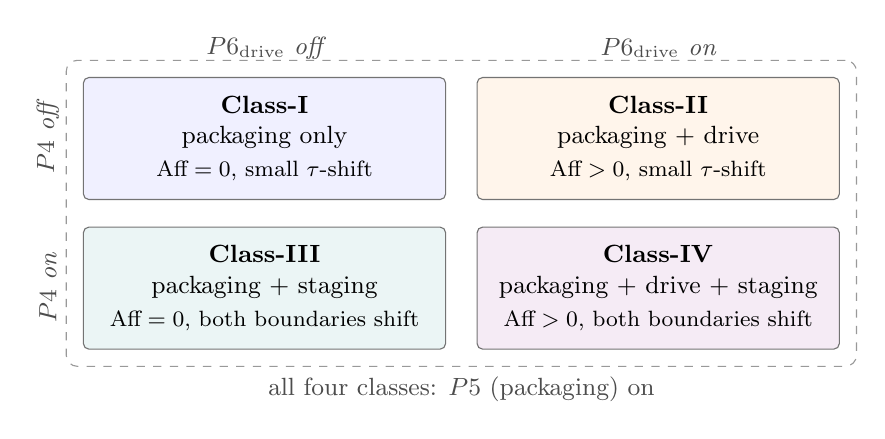
\begin{tikzpicture}[
  cell/.style={draw=black!55, rounded corners=2pt, minimum width=4.6cm, minimum height=1.55cm, align=center, font=\small},
  ax/.style={font=\small\itshape, text=black!70}]
\node[cell, fill=blue!6]   (c1) at (0,0)     {\textbf{Class-I}\\ packaging only\\[1pt] \footnotesize Aff${}=0$, small $\tau$-shift};
\node[cell, fill=orange!8] (c2) at (5.0,0)   {\textbf{Class-II}\\ packaging + drive\\[1pt] \footnotesize Aff${}>0$, small $\tau$-shift};
\node[cell, fill=teal!8]   (c3) at (0,-1.9)  {\textbf{Class-III}\\ packaging + staging\\[1pt] \footnotesize Aff${}=0$, both boundaries shift};
\node[cell, fill=violet!8] (c4) at (5.0,-1.9){\textbf{Class-IV}\\ packaging + drive + staging\\[1pt] \footnotesize Aff${}>0$, both boundaries shift};
\node[ax] at (0,1.15)   {$P6_{\mathrm{drive}}$ off};
\node[ax] at (5.0,1.15) {$P6_{\mathrm{drive}}$ on};
\node[ax, rotate=90] at (-2.75,0)    {$P4$ off};
\node[ax, rotate=90] at (-2.75,-1.9) {$P4$ on};
\node[draw=black!40, dashed, rounded corners=4pt, inner sep=6pt, fit=(c1)(c2)(c3)(c4)] (box) {};
\node[font=\small, text=black!70, anchor=north] at (box.south) {all four classes: $P5$ (packaging) on};
\end{tikzpicture}
\caption{The four classes as a $2\times 2$ grid. Packaging is required for a birth; drive (columns) and staging (rows) switch independently. The small text in each cell shows the signature of this paper's representative for that class. The general rule uses thresholds: drive is on for $\mathrm{Aff}_{\mathrm{ref}}\ge10^{-3}$ and off for $\mathrm{Aff}_{\mathrm{ref}}\le10^{-6}$ (Section~\ref{sec:observables-evidence}).}
\label{fig:taxonomy}
\end{figure}

Two points about this table matter for the rest of the paper.

\emph{The table is canonical, not exhaustive.} It lists the lowest-complexity combinations that are both motivated by the framework and measurable with the observables of Section~\ref{sec:observables-evidence}. We do not claim that no other kind of birth exists.

\emph{A staging signal is not the same as staging activation.} A system can show some sensitivity to the observation timescale without that sensitivity being strong enough to define a class. The Class-I and Class-II representatives both show a weak staging signal and are still not staging classes. We call the weak version a \emph{$P4$-like signal} and reserve \emph{$P4$ activation} for the strict version defined in Section~\ref{sec:observables-evidence}. This two-level rule is what keeps the table from collapsing whenever a boundary moves slightly.

\section{How the classes are measured}
\label{sec:observables-evidence}

This section sets out the finite-state setting, the three observable channels, and the rule that turns measurements into a class label. Everything is operational: the observables are computed on sampled parameter grids at finite system sizes, and the thresholds are conventions of this taxonomy rather than universal constants.

\subsection{Setting}

A system is a row-stochastic kernel $P$ on $n$ microstates. A \emph{lens} groups microstates into $k$ macrostates. We write it as an $n\times k$ zero--one matrix $Q$, with $Q_{ix}=1$ when microstate $i$ belongs to macrostate $x$. A \emph{lift} is a $k\times n$ stochastic matrix $U$ whose row $x$ is supported on the microstates of macrostate $x$, so that $UQ=I_k$. In the canonical analysis the lens has two equal blocks ($k=2$), chosen by hand from the known block structure of each family (the \emph{manual lens}), and the lift is uniform on each block.

Packaging is switched on gradually by mixing the dynamics with the ``package-and-redistribute'' kernel $QU$:
\[
P_\lambda=(1-\lambda)P+\lambda\,QU,\qquad \lambda\in[0,1].
\]
We call $\lambda$ the \emph{closure strength}. At $\lambda=1$ the dynamics is $QU$ itself. Because $UQ=I$, this kernel is idempotent, $(QU)^2=QU$. (This algebraic fact is the one mechanized statement used here; see Section~\ref{sec:exact-results}.) To observe the system at timescale $\tau\in\{1,2\}$ we use the \emph{empirical endomap}
\[
E=P_\lambda^{\tau}\,Q\,U,
\]
which runs the dynamics for $\tau$ steps, coarse-grains, and re-lifts.

\subsection{Three observable channels}

\paragraph{Packaging: closure error and objecthood.} A fully packaged description reproduces itself, so $E$ should be close to idempotent. The \emph{closure error} measures the largest row-wise failure of idempotence in total variation,
\[
\mathrm{CE}=\max_i \tfrac12\bigl\|E_{i\cdot}-(E^2)_{i\cdot}\bigr\|_1 .
\]
The \emph{objecthood order parameter} measures how well macrostates retain themselves. Let $B=U P_\lambda^{\tau} Q$ be the induced $k\times k$ macro kernel. A macrostate $x$ is retained with probability $B_{xx}$, so $\operatorname{tr}B$ is a soft count of stable objects, and for $k\ge2$
\[
M_{\mathrm{obj}}=\operatorname{clip}\!\Bigl(\tfrac{\operatorname{tr}B-1}{k-1},\,0,\,1\Bigr).
\]
For the two-block lens this is $\operatorname{clip}(\operatorname{tr}B-1,0,1)$. The idea that objects are picked out by closure has precedents outside dynamics, for example in perception and contour grouping \cite{marino_scholl_2005,wang_wang_kubota_2004}.

\paragraph{Drive: affinity.} Let $\pi$ be a stationary law of $P_\lambda^{\tau}$ and $J_{ij}=\pi_i(P_\lambda^{\tau})_{ij}$ the stationary flux. The \emph{affinity} is the stationary time-reversal divergence
\[
\mathrm{Aff}=D_{\mathrm{KL}}\bigl(J\,\|\,J^{\top}\bigr)=\sum_{i<j}\bigl(J_{ij}-J_{ji}\bigr)\log\frac{J_{ij}}{J_{ji}},
\]
that is, the entropy production per observed step \cite{seifert_2012,liang_pigolotti_2023}. It is zero exactly when the stationary process satisfies detailed balance, and it is $+\infty$ if some flux runs one way only. In this paper affinity is evaluated on the \emph{microstate} kernel at $\tau=1$. It is part of the declared measurement, not an arrow reconstructed from the macro description alone. The distinction is real: a biased four-cycle viewed through a parity lens has positive microscopic affinity but a reversible two-state macro kernel.

\paragraph{Staging: timescale shift of the boundaries.} Staging is detected by asking whether the birth moves when the observation timescale changes from $\tau=1$ to $\tau=2$ \cite{landim_2019,defenu_2021}. This uses the structural boundaries defined next.

\subsection{Boundaries}

Each observable is sampled on a declared $\lambda$ grid. The \emph{closure boundary} $\lambda_{\mathrm{CE}}$ is the first $\lambda$ at which CE falls to $0.025$, and the \emph{objecthood boundary} $\lambda_{M_{\mathrm{obj}}}$ is the first $\lambda$ at which $M_{\mathrm{obj}}$ reaches $0.90$. Both are located by linear interpolation between the last sample that misses the threshold and the first that meets it. If the threshold is already met at the first grid point, the boundary is \emph{left-censored}: we only know that it lies at or below that point, and we mark it as such. Birth requires both conditions together, so the structural reference boundary is the more conservative of the two,
\[
\lambda_{\mathrm{struct,ref}}=\max\bigl(\lambda_{\mathrm{CE}},\,\lambda_{M_{\mathrm{obj}}}\bigr),
\]
and we check that both thresholds hold simultaneously there on the interpolated curves. The drive reading at birth, $\mathrm{Aff}_{\mathrm{ref}}$, is the affinity curve interpolated linearly to $\lambda_{\mathrm{struct,ref}}$.

For staging we compute both boundaries at $\tau=1$ and at $\tau=2$ and record the shifts
\[
\Delta\lambda_{\mathrm{CE}}=\bigl|\lambda_{\mathrm{CE}}^{(\tau=2)}-\lambda_{\mathrm{CE}}^{(\tau=1)}\bigr|,\qquad
\Delta\lambda_{M_{\mathrm{obj}}}=\bigl|\lambda_{M_{\mathrm{obj}}}^{(\tau=2)}-\lambda_{M_{\mathrm{obj}}}^{(\tau=1)}\bigr|,
\]
together with a \emph{presence change} flag, which is raised when a boundary exists at one timescale and not at the other. The single staging coordinate used on the observable map is
\[
P4_{\mathrm{dual}}=\min\bigl(\Delta\lambda_{\mathrm{CE}},\,\Delta\lambda_{M_{\mathrm{obj}}}\bigr).
\]
It is large only if \emph{both} boundaries move.

\subsection{Decision rule}

Table~\ref{tab:rubric} gives the rule. Each primitive is assigned one of three states: on, off, or \emph{unknown}. Unknown is assigned whenever the evidence is missing or falls between the on and off thresholds. A system receives a class label only if all three states are known and the resulting signature matches a row of Table~\ref{tab:canonical-layer-birth-classes}. Otherwise it is reported as \emph{unclassified}. Missing evidence is never counted as evidence of absence: for example, a missing affinity reading does not make a system drive-free.

\begin{table}[tbp]
\centering
\small
\caption{Decision rule for the three switches. Shifts and boundaries are as defined in the text.}
\label{tab:rubric}
\begin{tabularx}{\linewidth}{@{}l Y Y@{}}
\toprule
Switch & On & Off \\
\midrule
$P5$ packaging & both boundaries exist and both thresholds (CE${}\le 0.025$, $M_{\mathrm{obj}}\ge 0.90$) hold at $\lambda_{\mathrm{struct,ref}}$ & $\min\mathrm{CE}>0.05$ and $\max M_{\mathrm{obj}}<0.85$ on the grid \\
$P6_{\mathrm{drive}}$ drive & $\mathrm{Aff}_{\mathrm{ref}}\ge 10^{-3}$ & $\mathrm{Aff}_{\mathrm{ref}}\le 10^{-6}$ \\
$P4$ staging & a presence change, or $\Delta\lambda_{\mathrm{CE}}\ge 0.15$ \emph{and} $\Delta\lambda_{M_{\mathrm{obj}}}\ge 0.15$ & both shifts measured, no presence change, and not on \\
\midrule
$P4$-like signal (not a class label) & \multicolumn{2}{l}{a presence change, or $\max(\Delta\lambda_{\mathrm{CE}},\Delta\lambda_{M_{\mathrm{obj}}})\ge 0.05$} \\
\bottomrule
\end{tabularx}
\end{table}

\subsection{Supporting quantities}

Three further kinds of quantity appear in the paper but play no part in assigning a class:
\begin{itemize}
  \item \emph{No-fake-arrow controls} test the drive channel by checking that reversible constructions are not labelled as driven (Section~\ref{sec:class-i-ii}).
  \item \emph{Shadow-ensemble susceptibility and Binder-type ratios} describe how $\Delta M_{\mathrm{obj}}$ fluctuates under small parameter perturbations that preserve the class (Section~\ref{sec:class-iii-iv}) \cite{fisher_barber_1972,binder_1981_prl}.
  \item \emph{Capacity/depth proxies} describe what happens after birth (Section~\ref{sec:observable-map-support}).
\end{itemize}

\paragraph{Lenses.} The class claims for Class-III and Class-IV are made for the manual lens. We also report two automatic lenses, a spectral sign-pattern lens and a diffusion-quantile lens, as a robustness test. These lenses do not enter the definitions \cite{mardt_noe_2021,nitskansky_clein_raveh_2026,sixbirds_lay_stone}.

\section{Exact results}
\label{sec:exact-results}

Most of the evidence in this paper is computational. This section collects the parts that can be stated and checked exactly. They make it possible to verify the class labels of the four representatives without relying on floating-point thresholds. Proofs are in Appendix~\ref{app:proofs}.

\subsection{A closed form for the packaging observables}

Write $A=P_\lambda^{\tau}Q$ (an $n\times k$ stochastic matrix) and $B=UA$ (the $k\times k$ macro kernel). Then $E=AU$ and $E^2=ABU$.

\begin{proposition}[Packaging reduction]
\label{prop:packaging}
Because the rows of $U$ have disjoint supports and unit mass, $\|vU\|_1=\|v\|_1$ for every row vector $v\in\mathbb{R}^k$. Consequently
\[
\mathrm{CE}=\tfrac12\max_i\bigl\|A_{i\cdot}-(AB)_{i\cdot}\bigr\|_1 .
\]
For the two-block lens with uniform lift, let $a_i=A_{i0}$ and let $b_0$ and $b_1$ be the averages of $a_i$ over blocks $0$ and $1$. Then
\[
\mathrm{CE}=\max_i\bigl|a_i-a_ib_0-(1-a_i)b_1\bigr|,\qquad M_{\mathrm{obj}}=\operatorname{clip}(b_0-b_1,\,0,\,1).
\]
\end{proposition}

So both packaging observables are determined by one column of $A$. This is what allows them to be computed in exact rational arithmetic for kernels with rational entries.

\subsection{An exact lower bound on affinity}

\begin{proposition}[Reversal lower bound]
\label{prop:reversal}
For $a,b>0$, $(a-b)\log(a/b)\ge 2(a-b)^2/(a+b)$. Hence, if $P_\lambda$ is doubly stochastic and the affinity is evaluated with the uniform stationary law $\pi_i=1/n$, then
\[
\mathrm{Aff}\;\ge\;\frac{2}{n}\sum_{i<j}\frac{\bigl(p_{ij}-p_{ji}\bigr)^2}{p_{ij}+p_{ji}},
\]
where the sum runs over pairs with $p_{ij}+p_{ji}>0$, and $\mathrm{Aff}=+\infty$ if some pair has $p_{ij}>0=p_{ji}$. In particular a symmetric kernel has $\mathrm{Aff}=0$ exactly.
\end{proposition}

All four representative kernels, and their mixtures with the uniform two-block $QU$, are doubly stochastic (checked exactly), and their affinity is evaluated with the uniform law, so the bound applies at every grid point. (For a reducible chain other stationary laws exist, and the bound need not hold for them. The uniform law is the one used here.) The bound uses no logarithms and is therefore exact in rational arithmetic. Since $\mathrm{Aff}_{\mathrm{ref}}$ is a linear interpolation of sampled values, the same interpolation of the sampled lower bounds is a lower bound for $\mathrm{Aff}_{\mathrm{ref}}$.

\subsection{Exact certificates for the four representatives}

Using Propositions~\ref{prop:packaging} and~\ref{prop:reversal}, an independent rational implementation rebuilds each representative kernel from its declared decimal parameters, read as exact fractions. It then evaluates CE and $M_{\mathrm{obj}}$ at every grid point for $\tau=1,2$, locates the boundaries, checks the joint birth condition, bounds the affinity, and applies the decision rule of Table~\ref{tab:rubric}. The results are in Table~\ref{tab:certificates}. All ten (class, size) points receive their intended label. The floating-point production code agrees with the exact grid values to within $3\times10^{-15}$.

\begin{table}[tbp]
\centering
\small
\caption{Exact certificates. Boundaries are at $\tau=1$; the lower bound is on $\mathrm{Aff}_{\mathrm{ref}}$ (``$0$'' means the kernel is symmetric and the affinity is exactly zero). An asterisk marks a left-censored boundary (threshold already met at the first grid point). Every row receives its intended class label.}
\label{tab:certificates}
\setlength{\tabcolsep}{4.5pt}
\begin{tabular}{@{}llrcccccc@{}}
\toprule
Class & Representative & $N$ & $\lambda_{\mathrm{CE}}$ & $\lambda_{M_{\mathrm{obj}}}$ & $\mathrm{Aff}_{\mathrm{ref}}\ge$ & $\Delta\lambda_{\mathrm{CE}}$ & $\Delta\lambda_{M_{\mathrm{obj}}}$ & $P4$ \\
\midrule
I   & \texttt{class\_i\_reference}  & 32  & 0.8743 & 0.7625 & $0$ & 0.0616 & 0.1155 & off \\
II  & \texttt{class\_ii\_reference} & 32  & 0.5556 & 0.5000$^{*}$ & 0.0340 & 0.1895 & 0.0000 & off \\
III & \texttt{replicated\_portal\_sp4} & 16, 32, 64, 128 & 0.5617 & 0.1233 & $0$ & 0.2016 & 0.3826 & on \\
IV  & \texttt{\ldots\_sp4\_drive\_f} & 16  & 0.6075 & 0.2149 & 0.00164 & 0.1826 & 0.3529 & on \\
IV  & & 32  & 0.5609 & 0.1219 & 0.00220 & 0.2033 & 0.3896 & on \\
IV  & & 64  & 0.5333 & 0.0666 & 0.00296 & 0.2157 & 0.4106 & on \\
IV  & & 128 & 0.5181 & 0.0500$^{*}$ & 0.00363 & 0.2223 & 0.4082 & on \\
\bottomrule
\end{tabular}
\end{table}

The certificates cover the declared finite grids and sizes, the manual two-block lens, and the uniform lift. The boundaries are interpolated proxies on those grids, not continuum transition points. For Class-IV the certificate holds at the four sizes listed and says nothing about larger sizes. For Class-III we can say more.

\subsection{Class-III is the same at every size}

The Class-III representative belongs to a \emph{replicated-portal} family. The $n=8m$ states ($m\ge 2$) form two blocks of $m$ modules each. Every module has three mutually connected ``fast'' states and one ``portal'' state, and each portal is linked to one partner portal in the other block. The kernel is the symmetric weight matrix, completed on the diagonal to constant row sums and normalized.

\begin{proposition}[Size independence of the undriven family]
\label{prop:lumpability}
Group the microstates into four types: fast or portal, in block 0 or block 1. Then $P_\lambda$ is strongly lumpable to these types, with a $4\times4$ type kernel $R_\lambda$ that does not depend on $m$. Moreover $P_\lambda^{\tau}Q=H\,R_\lambda^{\tau}L$ for every $\tau\ge0$, where $H$ maps states to types and $L$ maps types to blocks. Consequently CE and $M_{\mathrm{obj}}$ are independent of $m$ for every $\lambda\in[0,1]$ and every $\tau$, and $\mathrm{Aff}=0$ exactly because $P_\lambda$ is symmetric.
\end{proposition}

The proposition turns the size-16 certificate into a statement about every admissible size $n=8m\ge16$. The Class-III representative has exactly the same boundaries, shifts, and label at every size, which is why the Class-III row of Table~\ref{tab:certificates} is identical across $N$. The argument does not carry over to Class-IV. There the added global directed cycle crosses module and block boundaries, so the four-type lumping fails, and indeed the Class-IV values in Table~\ref{tab:certificates} change with $N$.

\subsection{What is and is not mechanized}

The one statement proved in a proof assistant is the idempotence used above: if $UQ=1$ then $(QU)(QU)=QU$. It is proved in Lean~4 for an abstract monoid and for morphisms in a small category, and the proofs depend on no axioms. It explains why $\mathrm{CE}=0$ and $M_{\mathrm{obj}}=1$ at $\lambda=1$. It does \emph{not} formalize the taxonomy, the decision rule, or the rational certificates. Those are exact computations in Python, checked independently against the production code, and not machine-checked proofs.

\section{Class-I and Class-II: structure with and without drive}
\label{sec:class-i-ii}

Class-I and Class-II both form structure, so both have packaging switched on. They differ in one respect only: whether directed circulation is present when the structure forms. This is the cleanest contrast in the paper.

\paragraph{Representatives.} The Class-I representative is a reversible two-block kernel. It has $N=32$ states in two blocks of 16, uniform within-block weight $1$, and cross-block weight $0.25$. The kernel is symmetric. The Class-II representative is a biased ring on $N=32$ states with stay, forward, and backward weights $0.10$, $0.55$, and $0.35$. Both are analysed with the manual two-block lens. Table~\ref{tab:class-i-ii-summary} gives their readings, which coincide with the exact certificates of Table~\ref{tab:certificates}.

\begin{table}[tbp]
\centering
\small
\caption{Class-I and Class-II reference readings ($N=32$, manual lens, $\tau=1$). The asterisk marks a left-censored boundary. Affinity is the floating-point reading at $\lambda_{\mathrm{struct,ref}}$; the exact lower bound is in parentheses.}
\label{tab:class-i-ii-summary}
\setlength{\tabcolsep}{4pt}
\begin{tabular}{@{}lccccccc@{}}
\toprule
Class & $\lambda_{\mathrm{CE}}$ & $\lambda_{M_{\mathrm{obj}}}$ & $\lambda_{\mathrm{struct,ref}}$ & $\mathrm{Aff}_{\mathrm{ref}}$ & $\Delta\lambda_{\mathrm{CE}}$ & $\Delta\lambda_{M_{\mathrm{obj}}}$ & Label \\
\midrule
I  & 0.874 & 0.763 & 0.874 & $0$ (exact) & 0.062 & 0.115 & Class-I \\
II & 0.556 & 0.500$^{*}$ & 0.556 & $3.45\times10^{-2}$ ($\ge 3.40\times10^{-2}$) & 0.189 & 0.000 & Class-II \\
\bottomrule
\end{tabular}
\end{table}

\paragraph{Both form structure.} Each representative reaches CE${}\le0.025$ and $M_{\mathrm{obj}}\ge0.90$ on its grid, so packaging is on for both (Figure~\ref{fig:structural-curves}, first two columns). Class-II forms structure at smaller closure strength. Its objecthood threshold is already met at the first grid point, $\lambda=0.5$, so only an upper bound is known for $\lambda_{M_{\mathrm{obj}}}$. This does not affect the label, because the closure boundary at $0.556$ is resolved and is the larger of the two.

\begin{figure}[tbp]
\centering
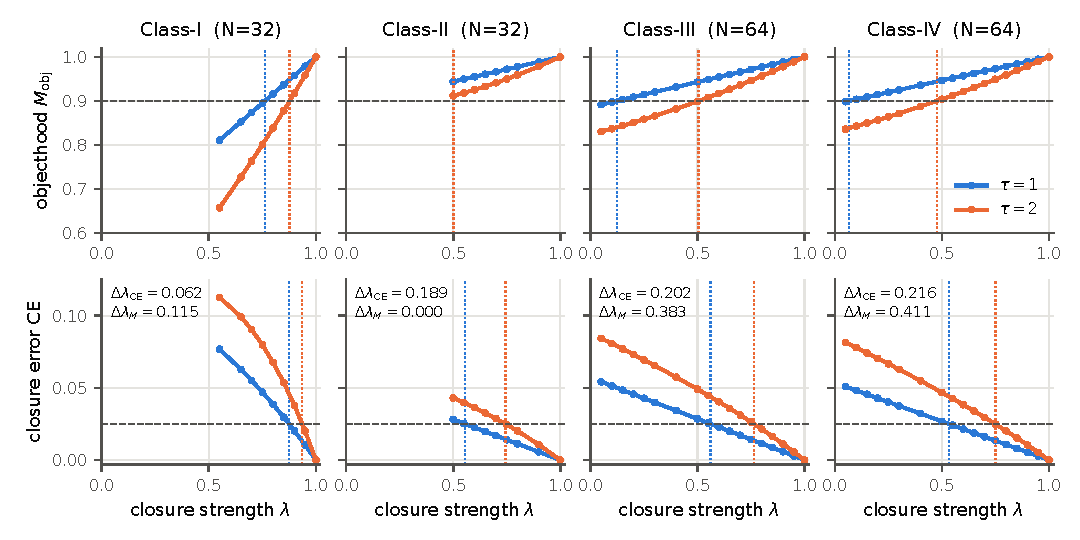
\includegraphics[width=\textwidth]{figures/structural_curves.pdf}
\caption{Exact structural curves of the four representatives (manual lens), at $\tau=1$ (blue) and $\tau=2$ (orange). Top row: objecthood, with threshold $0.90$. Bottom row: closure error, with threshold $0.025$. Dotted verticals mark the boundaries; the shifts between the two timescales are printed in each lower panel. Class-I and Class-II each have at least one small shift, so staging is off. Class-III and Class-IV have both shifts above $0.15$, so staging is on. Curve values are exact rationals at the grid points.}
\label{fig:structural-curves}
\end{figure}

\paragraph{Only Class-II carries drive.} The Class-I kernel and its mixtures with $QU$ are symmetric, so by Proposition~\ref{prop:reversal} the affinity is exactly zero at every $\lambda$. Class-II has $\mathrm{Aff}_{\mathrm{ref}}=3.45\times10^{-2}$ at its structural boundary. The exact lower bound, $3.40\times10^{-2}$, is more than an order of magnitude above the drive-on threshold of $10^{-3}$. Figure~\ref{fig:drive-curves} shows the affinity along the closure-strength axis. For Class-II it stays above $10^{-2}$ from $\lambda=0.5$ to $0.8$ and falls to zero at $\lambda=1$, where the dynamics becomes the symmetric kernel $QU$. Because the Class-I value is exactly zero, a ratio between the two affinities is meaningless. The relevant fact is the absolute gap: zero against a value well inside the drive-on region.

\begin{figure}[tbp]
\centering
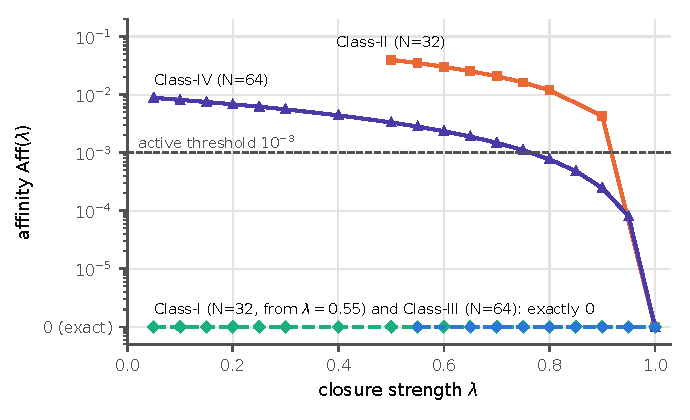
\includegraphics[width=0.66\textwidth]{figures/drive_curves.pdf}
\caption{Affinity along the closure-strength axis for the four representatives (manual lens, $\tau=1$). Class-I and Class-III are exactly zero on their whole grids (plotted on the floor). Class-II and Class-IV are positive until $\lambda=1$, where packaging replaces the dynamics by the symmetric kernel $QU$. The dashed line is the drive-on threshold.}
\label{fig:drive-curves}
\end{figure}

\paragraph{Staging is detectable but off.} Both representatives show some sensitivity to the timescale, so both have a $P4$-like signal (Table~\ref{tab:rubric}). Neither meets the strict rule. In Class-I both boundaries move, but by less than $0.15$ ($0.062$ and $0.115$). In Class-II the closure boundary moves by $0.189$ while the objecthood boundary does not move at all. This is exactly the case the two-level staging rule is designed for: a timescale effect that shows up in one channel only is recorded, but it does not make the birth a staging birth.

\paragraph{Controls against false arrows.} A drive axis is useful only if reversible systems are not mislabelled as driven. We ran two kinds of control (Table~\ref{tab:no-fake-arrow-summary}):
\begin{itemize}
  \item \emph{Reversible controls.} These are a reversible block kernel under the manual lens, the same kernel under the spectral lens, and a flat-mixing null kernel. All three have zero affinity and are not flagged as driven.
  \item \emph{Protocol-trap controls} \cite{sixbirds_protocol_trap}. Three reversible phase kernels are applied in a fixed cyclic order. When the ordered product is read as a single time-homogeneous kernel (the \emph{hidden-schedule} reading), it has affinity $0.058$ and is flagged as a driven candidate. Each constituent phase kernel, examined on its own (the \emph{phase-resolved} reading), has zero affinity and is not flagged.
\end{itemize}
The reversible controls show that the drive channel does not produce arrows out of reversible dynamics. The protocol trap shows that the channel reports on the kernel it is given: hiding the schedule produces an effective kernel that is genuinely non-reversible. This control does not construct the full autonomous process with an explicit phase register, so it is not a theorem that phase-aware handling always removes the arrow. Its purpose is narrower: to check that the audit separates the two readings as intended.

\begin{table}[tbp]
\centering
\small
\caption{No-fake-arrow controls.}
\label{tab:no-fake-arrow-summary}
\setlength{\tabcolsep}{4pt}
\begin{tabularx}{\linewidth}{@{}Y l l@{}}
\toprule
Control & Affinity & Flagged as driven? \\
\midrule
Protocol trap, hidden schedule (ordered product as one kernel) & 0.0576 & yes \\
Protocol trap, phase-resolved (each of the three phase kernels) & 0 & no \\
Reversible block kernel, manual lens & 0 & no \\
Reversible block kernel, spectral lens & 0 & no \\
Flat-mixing null kernel & 0 & no \\
\bottomrule
\end{tabularx}
\end{table}

\paragraph{Robustness.} Two further checks support the contrast. First, small-size robustness runs ($n=8$) swapped the manual lens for the spectral or the diffusion lens. For the reversible family the sampled birth window stayed at $[0.75,1]$. For the driven family it moved by one sampled interval, from $[0.5,0.75]$ to $[0.75,1]$, which is within the configured stability tolerance of one grid interval. This checks the approximate location of the structural window under a lens swap; it is not a full re-classification under those lenses. Second, in a scan over drive bias the affinity grows monotonically with the bias, while the structural boundary under the baseline $\tau=1$ analysis does not move. At $\tau=2$, however, some coupling between bias and structure is visible. In this sense drive behaves as a separate channel from packaging, but the separation is a property of the declared scan and is not proved in general.

\paragraph{Summary.} Class-I and Class-II are two distinct birth classes with the same structural switch and opposite drive switches. The difference is carried by an exact zero against a certified positive affinity, and the controls show that the drive channel does not invent arrows. This result needs no exponent fit, and it is the most robust result in the paper.

\section{Class-III and Class-IV: staging births}
\label{sec:class-iii-iv}

In Class-III and Class-IV the birth does more than form structure. Its location depends on the observation timescale, and it does so in both structural channels, so staging becomes part of the class identity. Class-III has no drive; Class-IV adds drive. These classes are harder to establish than Class-I and Class-II, and their claims are tied to the manual lens.

\paragraph{Representatives.} Both representatives come from the replicated-portal family described before Proposition~\ref{prop:lumpability}. They use fast weight $1.0$, fast--portal weight $0.02$, portal--cross weight $1.2$, and portal-self weight $4.0$. The Class-III kernel (\texttt{replicated\_portal\_sp4}) is this symmetric kernel. The Class-IV kernel (\texttt{replicated\_portal\_sp4\_drive\_f}) mixes it, with weight $0.12$, with a biased ring on all $N$ states (stay, forward, and backward weights $0.10$, $0.57$, and $0.33$). Both are analysed with the manual two-block lens on a 18-point grid from $\lambda=0.05$ to $1$.

\paragraph{Readings.} Table~\ref{tab:class-iii-iv-summary} gives the readings at $N=64$, the size used for the common map. Figure~\ref{fig:structural-curves} (last two columns) shows the curves. In both classes the closure and objecthood boundaries move by more than $0.15$ between $\tau=1$ and $\tau=2$, so $P4_{\mathrm{dual}}$ exceeds the strict threshold: $0.202$ for Class-III and $0.216$ for Class-IV. Class-III has exactly zero affinity. Class-IV has $\mathrm{Aff}_{\mathrm{ref}}=2.99\times10^{-3}$, with exact lower bound $2.96\times10^{-3}$.

\begin{table}[tbp]
\centering
\small
\caption{Class-III and Class-IV readings at $N=64$ (manual lens). Both have packaging and staging on.}
\label{tab:class-iii-iv-summary}
\setlength{\tabcolsep}{5pt}
\begin{tabular}{@{}llccccc@{}}
\toprule
Class & $P6_{\mathrm{drive}}$
  & $\lambda_{\mathrm{CE}}$
  & $\lambda_{M_{\mathrm{obj}}}$
  & $\lambda_{\mathrm{struct,ref}}$
  & $\mathrm{Aff}_{\mathrm{ref}}$
  & $P4_{\mathrm{dual}}$ \\
\midrule
III & off & 0.562 & 0.123 & 0.562 & $0$ (exact)          & 0.202 \\
IV  & on  & 0.533 & 0.067 & 0.533 & $2.99\times 10^{-3}$ & 0.216 \\
\bottomrule
\end{tabular}
\end{table}

\paragraph{Persistence across sizes.} Both labels hold at $N=16$, $32$, $64$, and $128$, and each of these points is certified exactly (Table~\ref{tab:certificates}). For Class-III, Proposition~\ref{prop:lumpability} gives more: the readings are identical at every admissible size $N=8m\ge16$, because the dynamics lumps exactly onto four state types. For Class-IV the readings drift with size. The structural boundary moves from $0.607$ to $0.518$, the affinity lower bound grows from $1.6\times10^{-3}$ to $3.6\times10^{-3}$, and $P4_{\mathrm{dual}}$ grows from $0.183$ to $0.222$. The label is unchanged, but we make no claim beyond $N=128$. At $N=128$ the Class-IV objecthood boundary is left-censored at the first grid point. The label is unaffected because the structural reference is set by the resolved closure boundary.

\paragraph{Why the two-level staging rule matters here.} The Class-I and Class-II representatives also show timescale sensitivity (Section~\ref{sec:class-i-ii}). What sets Class-III and Class-IV apart is that the shift is large in \emph{both} channels at once. Without the strict rule, any system with a moderate one-channel shift would be counted as a staging birth. With it, and in the absence of a boundary appearing or disappearing between timescales, staging becomes a class label only when the closure and objecthood descriptions both move with the timescale.

\paragraph{Shadow ensembles.} To see whether the staging classes support more than a yes/no label, we perturbed each representative's three portal weights by $\pm5\%$, one at a time. For Class-IV the four drive parameters are perturbed by $\pm5\%$ as well. We kept only perturbations that preserve the label at all four sizes. Every candidate passed, so the ensembles have 7 members (Class-III) and 15 members (Class-IV), counting the unperturbed kernel, at each of 18 values of $\lambda$ and each size. On these ensembles we compute the susceptibility $\chi=N\,\mathrm{Var}(\Delta M_{\mathrm{obj}})$ of the timescale difference $\Delta M_{\mathrm{obj}}=M_{\mathrm{obj}}(\tau{=}2)-M_{\mathrm{obj}}(\tau{=}1)$, together with a Binder-type moment ratio \cite{fisher_barber_1972,binder_1981_prl}.

Figure~\ref{fig:shadow-susceptibility} shows the result. The susceptibility peaks near $\lambda\approx0.4$--$0.5$, with peak values from $1.3\times10^{-5}$ ($N=16$) to $1.0\times10^{-4}$ ($N=128$) for Class-III and from $4.9\times10^{-6}$ to $4.8\times10^{-5}$ for Class-IV. These numbers must be read with care. The ensemble is a distribution over perturbed parameters, not a thermodynamic ensemble. For Class-III the distribution of $\Delta M_{\mathrm{obj}}$ is exactly the same at every size (Proposition~\ref{prop:lumpability}), so $\chi$ grows exactly in proportion to $N$, because of the factor $N$ in its definition, and not because of any critical behaviour. For Class-IV the peak value of $\chi/N$ rises only slowly, by about $21\%$ from $N=16$ to $128$, although at the smallest $\lambda$ the relative increase is larger. The Binder-type ratio is within $0.01$ of $2/3$ at every point except $\lambda=1$, where all members coincide and the ratio is undefined. The value $2/3$ is what one expects for a narrow distribution centred away from zero. The panels are therefore a usable description of how $\Delta M_{\mathrm{obj}}$ fluctuates within a class, but they provide no evidence for critical exponents.

\begin{figure}[tbp]
\centering
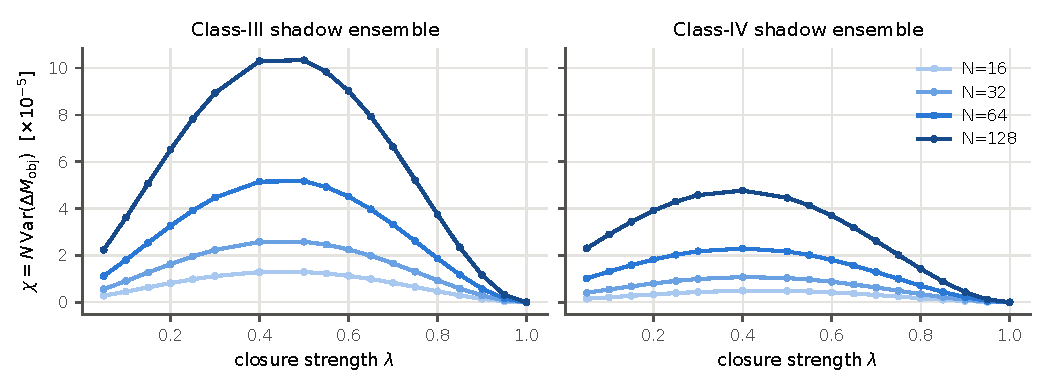
\includegraphics[width=\textwidth]{figures/shadow_susceptibility.pdf}
\caption{Shadow-ensemble susceptibility of the timescale difference $\Delta M_{\mathrm{obj}}$ under small class-preserving perturbations (manual lens). For Class-III the underlying distribution does not depend on $N$, so the curves differ only by the factor $N$ in $\chi$. For Class-IV, $\chi/N$ grows slightly with $N$. These are perturbation ensembles, not thermodynamic ones, and are not used for exponent claims.}
\label{fig:shadow-susceptibility}
\end{figure}

\paragraph{Lens dependence.} Replacing the manual lens with either automatic lens removes the staging label (Table~\ref{tab:class-iii-iv-lens-caveat}). The two automatic lenses give identical readings here. For Class-III they still find structure and no drive, so the birth is relabelled Class-I at both tested sizes. For Class-IV the result is worse. At $N=32$ the drive reading at the shifted boundary falls between the off and on thresholds, so drive is unknown and the system is unclassified. At $N=128$ drive is on but the objecthood shift vanishes, giving Class-II. In both classes the automatic lenses lose staging \emph{activation}, which is the defining feature. Class-III loses even the weak $P4$-like signal. Class-IV keeps a $P4$-like signal, because one of its shifts still exceeds $0.05$, but never both shifts above $0.15$.

\begin{table}[tbp]
\centering
\small
\caption{Class-III and Class-IV representatives under the two automatic lenses (spectral sign-pattern and diffusion-quantile; their readings coincide). The manual-lens label is confirmed at both sizes.}
\label{tab:class-iii-iv-lens-caveat}
\setlength{\tabcolsep}{4pt}
\begin{tabularx}{\linewidth}{@{}l c l l l Y@{}}
\toprule
Representative & $N$ & Manual & Automatic & $P5$ / $P6_{\mathrm{drive}}$ & Staging \\
\midrule
Class-III & 32  & Class-III & Class-I      & on / off     & no shift in either channel \\
Class-III & 128 & Class-III & Class-I      & on / off     & no shift in either channel \\
Class-IV  & 32  & Class-IV  & unclassified & on / unknown & shifts $0.119$, $0.232$: one below $0.15$ \\
Class-IV  & 128 & Class-IV  & Class-II     & on / on      & objecthood shift $0$ \\
\bottomrule
\end{tabularx}
\end{table}

\paragraph{What is established.} In the manual-lens channel, staging births exist with and without drive. They are certified exactly at four sizes and, for Class-III, at every admissible size, and they are separated from each other and from Class-I and Class-II by the measured observables. What is not established is that these labels survive an arbitrary change of coarse-graining. The two automatic lenses we tested do not reproduce them. Section~\ref{sec:discussion} returns to what this does and does not imply.

\section{All four classes on one map}
\label{sec:observable-map-support}

The preceding sections looked at the classes in pairs. Here all four representatives are measured at the same size, $N=64$, with the manual lens, and placed in one coordinate system. The coordinates are the three readings that enter the decision rule:
\begin{itemize}
  \item the structural boundary $\lambda_{\mathrm{struct,ref}}$ (horizontal axis);
  \item the affinity at that boundary, $\log_{10}\mathrm{Aff}_{\mathrm{ref}}$, clipped at $-12$ so that exact zeros can be drawn (vertical axis);
  \item the staging coordinate $P4_{\mathrm{dual}}$ (filled markers for staging on, hollow for off).
\end{itemize}
All coordinates are recomputed from the representative kernels at $N=64$. The Class-I and Class-II readings therefore differ slightly from the $N=32$ values of Section~\ref{sec:class-i-ii}.

\begin{table}[tbp]
\centering
\small
\caption{Observable-map coordinates at $N=64$ (manual lens, $\tau=1$ boundaries). An asterisk marks a left-censored boundary.}
\label{tab:four-class-observable-coordinates}
\setlength{\tabcolsep}{4.5pt}
\begin{tabular}{@{}llccccc@{}}
\toprule
Class & Representative
  & $\lambda_{\mathrm{CE}}$
  & $\lambda_{M_{\mathrm{obj}}}$
  & $\lambda_{\mathrm{struct,ref}}$
  & $\mathrm{Aff}_{\mathrm{ref}}$
  & $P4_{\mathrm{dual}}$ \\
\midrule
I   & \texttt{class\_i\_reference}   & 0.871 & 0.756 & 0.871 & $0$ (exact)          & 0.063 \\
II  & \texttt{class\_ii\_reference}  & 0.500$^{*}$ & 0.500$^{*}$ & $\le 0.500$ & $4.23\times 10^{-2}$ & 0.000 \\
III & \texttt{replicated\_portal\_sp4} & 0.562 & 0.123 & 0.562 & $0$ (exact)          & 0.202 \\
IV  & \texttt{\ldots\_sp4\_drive\_f}   & 0.533 & 0.067 & 0.533 & $2.99\times 10^{-3}$ & 0.216 \\
\bottomrule
\end{tabular}
\end{table}

\begin{figure}[tbp]
\centering
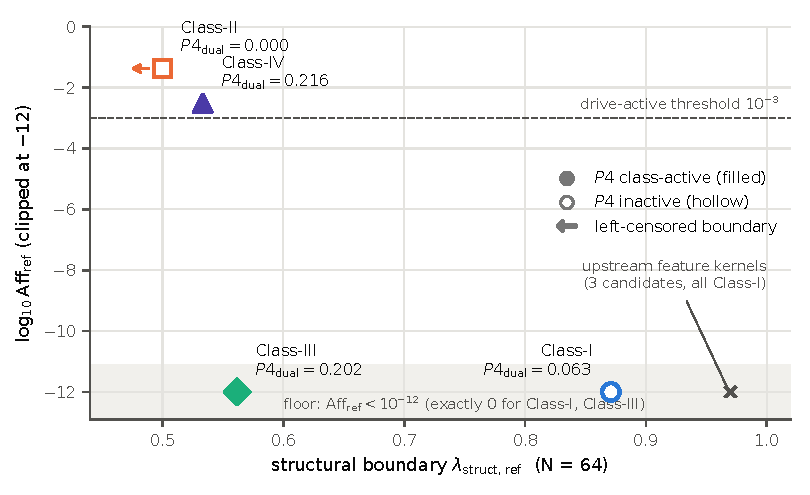
\includegraphics[width=0.8\textwidth]{figures/observable_map.pdf}
\caption{The four representatives on a common observable map ($N=64$, manual lens). Horizontal: structural boundary. Vertical: affinity at the boundary (log scale; the shaded floor holds readings below $10^{-12}$, which for Class-I and Class-III are exact zeros). Filled markers have staging on, hollow markers have it off. The Class-II boundary is left-censored (arrow). Grey crosses: three kernels built from upstream compiled features, all classified Class-I.}
\label{fig:four-class-observable-map}
\end{figure}

Table~\ref{tab:four-class-observable-coordinates} and Figure~\ref{fig:four-class-observable-map} show the result. The drive axis splits the classes into two pairs: Class-II and Class-IV sit above the drive-on threshold, and Class-I and Class-III sit at exact zero. The staging coordinate splits them the other way: Class-III and Class-IV have $P4_{\mathrm{dual}}\approx0.2$, while Class-I and Class-II have $0.063$ and $0$. Neither coordinate separates all four classes on its own, but together they do. The structural boundary does not separate the classes, but it records where each birth happens. Class-I forms structure latest ($\lambda\approx0.87$). The displayed boundaries of the other three lie between $0.50$ and $0.56$, but for Class-II the value $0.50$ is only an upper bound.

At $N=64$ the Class-II boundary is left-censored. Both structural thresholds are already met at the first grid point, $\lambda=0.5$, so the boundary is known only to lie at or below $0.5$. Its true position on the horizontal axis could be well to the left of the plotted point. This affects where Class-II sits along that axis but not its class. The affinity reading is taken at the censored boundary, $\lambda=0.5$, and is $4.23\times10^{-2}$, far above the drive-on threshold. The affinity curve decreases with $\lambda$ (Figure~\ref{fig:drive-curves}), so any boundary further to the left would give a larger reading.

This map is the main synthetic result of the paper. Its value is that it is built directly from the observables that define the classes. It does not depend on exponent fits, which remain unreliable here (Appendix~\ref{app:negative-results}). It is a map of four representative systems, not a phase diagram of the parameter space.

\subsection{Upstream feature kernels}

To test whether the observables can be computed on systems from outside our synthetic families, we built kernels from a vendored copy of the upstream Six-Birds closure library. Three symbolic instances (\texttt{tau\_conflict}, \texttt{audit\_sector}, and \texttt{audit\_partition\_loop}) were compiled by the library's own compiler into substrates with 22, 50, and 54 states. From each compiled substrate we constructed a kernel: a row-normalized Gram matrix of the compiled features with a boost within each sector, mixed with an artificial preference-gradient term. This is therefore a kernel derived from upstream features, not the upstream system's native dynamics.

All three kernels run through the same pipeline and receive the label Class-I. They have structural boundaries near $\lambda\approx0.97$, affinities of order $10^{-23}$ (drive off), and $P4_{\mathrm{dual}}\approx0.014$ (staging off, though a weak $P4$-like signal is present). They appear as the grey crosses in Figure~\ref{fig:four-class-observable-map}. The result shows that the map can be applied to kernels from another codebase. It does not show that the upstream system realizes the other three classes, and the ``high'' confidence reported by the bridge is a heuristic, not a statistical statement.

\subsection{Capacity and depth after birth}

We also measured post-birth proxies for each representative: the remaining closure-strength headroom $1-\lambda_{\mathrm{struct,ref}}$, how long (in $\tau$) the structural targets survive, the area under the objecthood curve across $\tau$, and a combined capacity--depth index. Under the packaging control these proxies are not independent of the birth location. At $\lambda=1$ the dynamics is the idempotent kernel $QU$, so for every positive $\tau$ we have $\mathrm{CE}=0$ and $M_{\mathrm{obj}}=1$, and with the uniform two-block lift also $\mathrm{Aff}=0$. Depth survival and objecthood area therefore saturate at the same values for all four classes, and the combined index reduces algebraically to $(1-\lambda_{\mathrm{birth}})\cdot\tau_{\max}$, where $\tau_{\max}=8$ is the largest sampled timescale and $\lambda_{\mathrm{birth}}$ is the structural boundary measured by the capacity campaign. In other words, the capacity index is a rescaled copy of a structural boundary proxy. That proxy is measured on campaign-specific grids: the scaling-campaign grids for Class-I and Class-II and the full-campaign grids for Class-III and Class-IV. For Class-II these differ from the map grid. There the grid starts at $\lambda=0.4$, and the Class-II capacity reference ($0.4$ at $N=64$) is again left-censored. Consistent with this, it does not line up cleanly with either the drive axis or the staging axis. We report it as a description of what happens after birth, not as a classifier, and we draw no further conclusion from it.

\section{Discussion}
\label{sec:discussion}

\paragraph{What the paper establishes.} Layer births can be classified by which primitives switch on at birth. With packaging required, and drive and staging as independent switches, there are four canonical classes. Each class has an explicit representative that the decision rule labels correctly. For all four, the label is certified exactly on the declared grids. On a common observable map the four classes occupy distinct regions. None of this depends on critical exponents.

\paragraph{How strong each part is.} The parts of the result do not carry equal weight.
\begin{itemize}
  \item \emph{Class-I versus Class-II} is the strongest part. The two classes share the structural switch and differ in drive. The difference is an exactly zero affinity against a certified positive one, and the controls confirm that the drive channel does not turn reversible dynamics into a false arrow.
  \item \emph{Class-III} is strong within its channel. Its label is certified exactly, and Proposition~\ref{prop:lumpability} shows that it holds at every admissible size of the undriven family, not just the sizes we sampled.
  \item \emph{Class-IV} is certified at four sizes (16--128). Its readings drift with size, and we make no claim beyond the sampled sizes.
  \item \emph{Both staging classes} depend on the manual lens. Under the two automatic lenses we tested, staging activation disappears (a weaker $P4$-like signal survives for Class-IV only), and the labels revert to Class-I, Class-II, or unclassified.
\end{itemize}

\paragraph{How to read the lens dependence.} One reading is that the manual lens, which follows the known block structure of the family, is the right description, and that the automatic lenses group states in ways that hide the slow cross-block channel responsible for staging. Another reading is that staging, as measured here, is a property of the pair (system, lens) rather than of the system alone. Our data do not decide between these readings. What they do show is that staging births are more delicate to measure than drive births, and that any claim about them should state the lens. A natural next step is to search for automatic lenses that recover the manual partition, or to characterize the lenses under which staging is preserved.

\paragraph{The two-level staging rule.} Requiring both structural boundaries to move ($P4_{\mathrm{dual}}\ge0.15$), rather than either one, does real work. Without it, the Class-II representative, whose closure boundary moves by $0.19$, would be counted as a staging birth. With it, and absent a boundary that appears or disappears between timescales, staging becomes a class label only when the closure and objecthood descriptions move together. The weaker one-channel signal is still recorded, as a $P4$-like signal.

\paragraph{What the negative results say.} Two lines of investigation failed in instructive ways (Appendix~\ref{app:negative-results}). The holonomy experiments did not produce a clean crossover field: route mismatch either produced nothing class-relevant or acted only by leaking into the drive channel. This supports the decision, made on theoretical grounds, not to treat $P3$ as a class axis \cite{sixbirds_protocol_trap,liang_pigolotti_2023}. The finite-size-scaling fits did not stabilize. Exponent estimates moved with the fit grid and sat on the grid boundary, and adding a size did not help \cite{fisher_barber_1972,binder_1981_prl,ardourel_bangu_2023}. We therefore make no exponent claims. The observable map is more reliable than the fits because it is built from the class-defining observables themselves, not from the minimum of an unstable collapse objective.

\paragraph{Staging classes as a place to look.} Class-III and Class-IV are the first classes in this taxonomy in which competing timescales are part of the birth's identity rather than a small correction. That makes them natural candidates for studying post-birth organization driven by competing timescales. This is a suggestion for future work. The present evidence does not demonstrate it.

\paragraph{Open problems.} Four problems stand out:
\begin{enumerate}
  \item make the staging classes robust beyond the manual lens, or characterize exactly which lenses preserve them;
  \item extend the Class-IV certificate beyond $N=128$, perhaps with a lumping argument adapted to the directed cycle;
  \item decide whether the four classes are distinct universality classes in the asymptotic sense, which will need finite-size data that support stable fits;
  \item obtain upstream kernels from native dynamics rather than compiled features, and find upstream realizations of Class-II through Class-IV.
\end{enumerate}

\section{Conclusion}
\label{sec:conclusion}

We asked whether layer births come in different kinds that can be told apart by measurement. Within the Six-Birds framework the answer supported here is yes: at least four. All four classes form structure (packaging). They differ in whether drive is present at birth and whether the birth moves with the observation timescale (staging).

Each class has an explicit finite representative, and its label is certified exactly on the declared grids. The undriven staging class is certified at every admissible size. The structure-with-drive versus structure-without-drive contrast (Class-I versus Class-II) is the most robust result: it rests on an exactly zero versus a clearly positive affinity, and controls show that the drive channel does not create false arrows. The staging classes are confirmed under the manual lens only.

At a common size the four classes occupy distinct regions of a three-coordinate observable map built from the same quantities that define them. Capacity/depth proxies turn out to be a rescaling of the structural boundary and are not classifiers. Kernels built from upstream compiled features can be placed on the map and land in Class-I.

The result is a vocabulary and a set of measurements, not a theory of universality classes. Whether these four classes remain distinct in the asymptotic, exponent-level sense is the next question, and this paper does not answer it.


\appendix
\section{Proofs of the exact results}
\label{app:proofs}

Throughout, $P$ is an $n\times n$ row-stochastic matrix, $Q$ is the $n\times k$ zero--one matrix of a surjective lens, and $U$ is a $k\times n$ stochastic lift with row $x$ supported on the fiber of $x$, so $UQ=I_k$. We set $P_\lambda=(1-\lambda)P+\lambda QU$, $A=P_\lambda^{\tau}Q$, $B=UA$, and $E=AU$.

\begin{proof}[Proof of Proposition~\ref{prop:packaging}]
Let $v\in\mathbb{R}^k$. The vector $vU$ places the mass $v_xU_{xj}$ on microstate $j$ in fiber $x$. Fibers are disjoint and $U_{xj}\ge0$, so $\|vU\|_1=\sum_x|v_x|\sum_jU_{xj}=\sum_x|v_x|=\|v\|_1$. Now $E^2=AUAU=ABU$. Hence $E_{i\cdot}-(E^2)_{i\cdot}=(A_{i\cdot}-(AB)_{i\cdot})U$, and the isometry gives the first formula.

For $k=2$ with uniform lift on two blocks of equal size $h$, each row of $A$ is $(a_i,1-a_i)$. The macro kernel has entries $B_{00}=b_0$, $B_{01}=1-b_0$, $B_{10}=b_1$, $B_{11}=1-b_1$, where $b_0$ and $b_1$ are the block averages of $a$. Then $(AB)_{i0}=a_ib_0+(1-a_i)b_1$. Both rows sum to one, so $A_{i\cdot}-(AB)_{i\cdot}=(d_i,-d_i)$ with $d_i=a_i-a_ib_0-(1-a_i)b_1$, and half its $\ell_1$ norm is $|d_i|$. Finally $\operatorname{tr}B-1=b_0+(1-b_1)-1=b_0-b_1$, which gives $M_{\mathrm{obj}}=\operatorname{clip}(b_0-b_1,0,1)$ for $k=2$.
\end{proof}

\begin{proof}[Proof of Proposition~\ref{prop:reversal}]
Let $x=a/b\ge1$ and $g(x)=\log x-2(x-1)/(x+1)$. Then $g(1)=0$ and $g'(x)=(x-1)^2/\bigl(x(x+1)^2\bigr)\ge0$, so $g\ge0$ on $[1,\infty)$. Multiplying $g(a/b)\ge0$ by $a-b\ge0$ gives $(a-b)\log(a/b)\ge2(a-b)(a-b)/(a+b)$. The case $a<b$ follows by exchanging $a$ and $b$, since both sides are symmetric. With the uniform stationary law, $J_{ij}=p_{ij}/n$. Each pair term of $D_{\mathrm{KL}}(J\|J^{\top})$ is nonnegative and bounded below as stated, and a pair with flux in one direction only contributes $+\infty$. A symmetric kernel has $J=J^{\top}$, hence zero divergence. The uniform law is stationary exactly when $P_\lambda$ is doubly stochastic. The bound is stated for this law: a reducible chain may have other stationary laws, for which it can fail. For the representatives this holds because $P$ is doubly stochastic and, for the uniform two-block lift, $QU$ is symmetric and doubly stochastic. Both facts are checked in exact arithmetic.
\end{proof}

\begin{proof}[Proof of Proposition~\ref{prop:lumpability}]
Let $n=8m$, $m\ge2$, so each block has $m$ modules of three fast states and one portal. Denote the edge weights by $f$ (fast--fast), $g$ (fast--portal), $c$ (portal--cross-block portal), and $s$ (portal self-loop). Let $D=\max(2f+g,\,3g+c+s)>0$. The constructor adds $D-(2f+g)$ to each fast diagonal and $D-(3g+c+s)$ to each portal diagonal, then divides by $D$, which gives a symmetric stochastic $P$.

Let $H$ be the $n\times4$ zero--one matrix sending each state to its type $(\text{fast}_0,\text{portal}_0,\text{fast}_1,\text{portal}_1)$. Every fast state sends total probability $g/D$ to its portal and $1-g/D$ to fast states of its own block. Every portal sends $3g/D$ to its fast states, $c/D$ to its partner portal, and $1-(3g+c)/D$ to itself. None of these totals depends on $m$, so $PH=HT$ with
\[
T=\begin{pmatrix}
1-g/D & g/D & 0 & 0\\
3g/D & 1-(3g+c)/D & 0 & c/D\\
0 & 0 & 1-g/D & g/D\\
0 & c/D & 3g/D & 1-(3g+c)/D
\end{pmatrix}.
\]
Let $L$ be the $4\times2$ matrix sending types to blocks, and let $V$ be the $2\times4$ lift that gives each block its fast and portal types with weights $(3/4,1/4)$. Each block has $3m$ fast states and $m$ portals, so the uniform lift satisfies $UH=V$, and $Q=HL$. Therefore $(QU)H=HLUH=HLV$, and
\[
P_\lambda H=H R_\lambda,\qquad R_\lambda=(1-\lambda)T+\lambda LV,
\]
which is independent of $m$. By induction $P_\lambda^{\tau}H=HR_\lambda^{\tau}$, so $A=P_\lambda^{\tau}Q=HR_\lambda^{\tau}L$. The rows of $A$ depend only on the type of the state, and $UA=VR_\lambda^{\tau}L$ is independent of $m$. By Proposition~\ref{prop:packaging}, CE is the maximum of $\tfrac12\|A_{i\cdot}-(AUA)_{i\cdot}\|_1$ over states, and hence over the four types, all of which occur for $m\ge2$. $M_{\mathrm{obj}}=\operatorname{clip}(\operatorname{tr}(UA)-1,0,1)$. Neither depends on $m$. This holds for every $\lambda$ and $\tau$, so the boundaries, their shifts, and the presence or absence of crossings on any fixed grid are the same for all $m$. Finally, $P$ and $QU$ are symmetric, so $P_\lambda$ is symmetric and $\mathrm{Aff}=0$ by Proposition~\ref{prop:reversal}. This holds even when $P$ is reducible.
\end{proof}

\begin{remark}
The argument uses strong lumpability of $P_\lambda$ itself. It does not assume that arbitrary micro observables descend through the two-block lens. Adding the global directed ring of the Class-IV family breaks this lumping. States of the same type no longer have the same transition probabilities to the four types: for example, along the ring only the last fast state of each module steps directly into a portal, and only the last portal of each block steps into the other block. The argument therefore does not extend to the driven family.
\end{remark}

\section{Rubric and representative details}
\label{app:metrics-rubric}

This appendix records the parameters behind the decision rule of Table~\ref{tab:rubric} and the representative kernels. The thresholds are conventions of this taxonomy. The claims of the paper concern their consistent use on the declared grids, not the absence of other reasonable choices.

\paragraph{Thresholds.} Packaging targets: CE${}\le0.025$ and $M_{\mathrm{obj}}\ge0.90$. Packaging off: $\min\mathrm{CE}>0.05$ and $\max M_{\mathrm{obj}}<0.85$ on the grid. Drive on: $\mathrm{Aff}_{\mathrm{ref}}\ge10^{-3}$. Drive off: $\mathrm{Aff}_{\mathrm{ref}}\le10^{-6}$. $P4$-like signal: a presence change, or a largest shift of at least $0.05$. $P4$ on: a presence change, or both shifts at least $0.15$. $P4$ off: both shifts measured, no presence change, and the on condition fails. For packaging and drive, readings between the on and off thresholds are unknown. For every switch, missing evidence is unknown. A system with any unknown switch is unclassified. In addition to the main reading $\mathrm{Aff}_{\mathrm{ref}}$, the pipeline records affinity onset locations at $10^{-3}$, $10^{-2}$, and $5\times10^{-2}$ as diagnostics. These onsets do not enter the rule.

\paragraph{Boundary conventions.} Boundaries are first-hit locations, linearly interpolated between the last miss and the first hit. A hit at the first grid point is recorded as left-censored. Duplicate grid coordinates and missing (NaN) readings are rejected. Infinite readings are allowed: an infinite affinity, which arises from one-way flux, counts as drive on, and at a support singularity only the sampled hit is used for a boundary. The structural reference $\max(\lambda_{\mathrm{CE}},\lambda_{M_{\mathrm{obj}}})$ is accepted only if both thresholds hold together there on the interpolated curves. This matters for non-monotone curves, where one threshold may be met early and lost again later. $\mathrm{Aff}_{\mathrm{ref}}$ is the linear interpolation of the sampled affinity at the $\tau=1$ structural reference.

\paragraph{Stationary laws.} Affinity requires a stationary law. The pipeline computes it with a solver that decomposes the chain into communicating classes. It handles periodic and reducible kernels, assigns zero mass to transient states, and rejects any result whose balance residual exceeds a stated tolerance. Unconverged power iterates are never passed on as stationary laws. This matters in practice: twenty plain power steps on the reversible chain $\bigl(\begin{smallmatrix}0&1&0\\ 1/4&0&3/4\\ 0&1&0\end{smallmatrix}\bigr)$ give an apparent affinity of $0.23$, but its true stationary law $(1/8,1/2,3/8)$ gives zero. For the exact certificates the stationary law is uniform, and this is verified exactly (Proposition~\ref{prop:reversal}).

\paragraph{Representative kernels and grids.} Table~\ref{tab:representatives} lists the representative kernels and grids.

\begin{table}[tbp]
\centering
\small
\caption{Representative kernels. All use the manual two-block lens, uniform lift, and $\tau\in\{1,2\}$.}
\label{tab:representatives}
\begin{tabularx}{\linewidth}{@{}l L{0.43\linewidth} Y@{}}
\toprule
Class & Kernel & $\lambda$ grid; sizes \\
\midrule
I   & two equal blocks; within-block weight $1$, cross-block $0.25$, no self-loop & $\{0.55,0.65,0.70,\dots,0.95,1\}$; $N=32$ (map: 64) \\
II  & ring; stay $0.10$, forward $0.55$, backward $0.35$ & $\{0.50,0.55,\dots,0.80,0.90,1\}$; $N=32$ (map: 64) \\
III & replicated portals; $f=1$, $g=0.02$, $c=1.2$, $s=4$ & 18 points, $0.05$--$1$; $N=16,32,64,128$ \\
IV  & Class-III kernel mixed (weight $0.12$) with a ring of stay $0.10$, forward $0.57$, backward $0.33$ & same as III \\
\bottomrule
\end{tabularx}
\end{table}

\paragraph{Lenses.} The manual lens splits each family into its two declared blocks. The two automatic lenses are built from a spectral coordinate. The left eigenpairs of $P^{\tau}$ (eigenpairs of $(P^{\tau})^{\top}$) are sorted by decreasing modulus, with ties broken by real part, then imaginary part, then index. Each eigenvector is replaced by its real part, and its sign is fixed so that its largest-magnitude entry is nonnegative. The coordinate is the second vector in this order. For $k=2$ the spectral sign-pattern lens groups states by the sign of this coordinate and falls back to a quantile split if the signs do not give exactly two groups. The diffusion-quantile lens splits states at the median of the same coordinate. The ordering is a deterministic convention: when the leading eigenvalue is degenerate, as for the reducible undriven portal kernel, or the selected eigenvalue is complex, as for the driven portal kernel, the coordinate is a convention-dependent choice, not a canonical slow mode. For the staging representatives the two constructions give the same readings. Both automatic lenses are used only in the robustness tests.

\paragraph{Lift ablations.} When a robustness run replaces the uniform lift (for example by a prototype or stationary-weighted lift), the same lift is used in every packaging observable as well as in the control $P_\lambda$. All canonical results use the uniform lift.

\section{Negative results and limits}
\label{app:negative-results}

Several stronger claims were tested and not retained. They are collected here because they define the scope of the main result. Table~\ref{tab:appendix-negative-constraints} summarizes them.

\paragraph{Holonomy is not a crossover field.} We tested whether route mismatch ($P3$) could shift the birth on its own. In the first family, one of the two cases with nonzero holonomy (the routed one) also picked up a small affinity ($1.7\times10^{-3}$), so its effect could not be separated from drive. In a refined family the affinity contamination was removed, but holonomy then produced no shift of the birth location, no change in the presence of the birth window, and only negligible change in curve shape (at most $3.7\times10^{-3}$). Route mismatch therefore either did nothing class-relevant or acted through the drive channel. This matches the framework's prior decision to keep $P3$ diagnostic \cite{sixbirds_protocol_trap}.

\paragraph{Exponents are not identifiable.} Finite-size-scaling collapse fits were run for the Class-I and Class-II families. The objective is a heuristic: a sum of pairwise curve mismatch, spread in raw $\lambda$, and a weighted slope penalty. It is not a pure collapse criterion. The best fits sat on the boundary of the search grid. On the enlarged grid the Class-I optimum moved to a trivial solution ($\lambda_c=1$ with both exponent coordinates zero), and the Class-II optimum sat at $\lambda_c=0.875$, also with both exponent coordinates zero. Adding a size of 128 changed neither picture. Where bootstrap intervals were reported they collapsed to a single point. They are conditional on the objective and the grid. Because the primary grouped observations have a single replicate per (size, $\lambda$), resampling supplies no sampling variability, so the intervals do not measure the precision of an exponent. We make no exponent claims.

\paragraph{Staging classes are lens-dependent.} See Table~\ref{tab:class-iii-iv-lens-caveat}. Under both automatic lenses, Class-III is relabelled Class-I. Class-IV becomes unclassified ($N=32$) or Class-II ($N=128$).

\paragraph{Capacity is not a classifier.} Under the packaging control, the capacity--depth index equals $(1-\lambda_{\mathrm{birth}})\,\tau_{\max}$, where $\lambda_{\mathrm{birth}}$ is the capacity campaign's structural boundary proxy (Section~\ref{sec:observable-map-support}). It carries no information beyond that structural coordinate, and its alignment with the drive and staging axes is mixed.

\paragraph{The upstream bridge is partial.} The three upstream-derived kernels are built from compiled features plus an artificial preference-gradient term, not from native upstream dynamics, and all three land in Class-I.

\begin{table}[tbp]
\centering
\small
\caption{Stronger claims that were tested and not retained.}
\label{tab:appendix-negative-constraints}
\begin{tabularx}{\linewidth}{@{}L{0.27\linewidth}L{0.2\linewidth}Y@{}}
\toprule
Claim tested & Outcome & Consequence \\
\midrule
Holonomy as an independent crossover field & not supported & $P3$ is not a class axis \\
Stable exponent extraction & not supported & no exponent or universality claims \\
Lens robustness of Class-III / IV & not supported for the two automatic lenses & staging claims are made for the manual lens \\
Capacity as a classifier & not supported; algebraically tied to the structural boundary & capacity reported as post-birth description only \\
Upstream realization of all four classes & not supported & bridge shown as an overlay of three Class-I kernels \\
Class-IV at all sizes & not established & certified at $N=16$--$128$ only \\
\bottomrule
\end{tabularx}
\end{table}

\section{Reproducibility and evidence ledger}
\label{app:reproducibility-ledger}

The code, configurations, exact audit, and figure scripts for this paper are in the public repository \url{https://github.com/ioannist/six-birds-layer-birth}. This appendix describes how the claims are tied to reproducible outputs.

\paragraph{Evidence ledger.} A reproducibility freeze, written to \path{results/freeze/reproducibility_freeze/}, maps each claim to the result bundles that support it. It reruns every producing workflow with result caches disabled and compares output hashes. Its key files are
\begin{quote}
\path{analysis/evidence_ledger.json}\\
\path{analysis/claim_coverage.json}\\
\path{analysis/reproducibility_summary.json}\\
\path{analysis/ready_for_writing_status.json}.
\end{quote}
Reproducing an output is not the same as reproducing a conclusion. The freeze therefore also runs configured checks of the specific scientific conclusions the paper draws from the supporting bundles, for example that the Class-III label holds at every checked size or that the four map coordinates are separable. A reproducible output with a false conclusion blocks readiness. In the current freeze all 14 assets (9 paper-critical and 5 supporting) reproduce, all declared conclusion checks pass, and all seven claim groups have their evidence. The three recorded caveats are the ones stated in the paper: lens fragility of the staging classes, the absence of exponent claims, and the limited upstream bridge.

\paragraph{Provenance.} Every cached computation is keyed by its full generating configuration and by a fingerprint of the package source, configuration files, orchestration scripts, vendored Python sources, dependency versions, and the Python and NumPy versions. Within one interpreter session a cached result is not reused for a different configuration or implementation. The fingerprint is computed once per process, so the interpreter must be restarted after fingerprinted sources or configurations are changed. Unavailable observations are stored as explicit nulls and infinities as explicit tags, and neither is replaced by zero. There is one documented exception. When every shadow-ensemble member coincides (at $\lambda=1$), the Binder-type ratio is undefined but is stored as $0$, and readers should treat those entries as undefined.

\paragraph{Exact audit.} The rational certificates of Section~\ref{sec:exact-results} are produced by \path{scripts/audit_canonical_mathematics.py}. The script uses an independent implementation (\path{src/layerbirth/exact_audit.py}) that rebuilds the kernels from the configuration files and does not read any cached result. Its output, \path{notes/math_review/canonical_exact_audit.json}, contains every grid value as an exact fraction, together with configuration hashes and the maximum discrepancy from the production code. The Lean statement of Section~\ref{sec:exact-results} is in the vendored library under \path{vendor/six-birds-pica-ma_snapshot_v71/lean}. Its axiom check is \path{notes/math_review/lean_axioms.lean}.

\paragraph{Tests and figures.} The test suite (245 tests) includes regression tests for each failure mode discussed in Appendix~\ref{app:metrics-rubric}, for example unconverged stationary laws, one-way flux, fallback affinities, and incomplete control panels. The figures are generated by \path{scripts/make_paper_figures.py} from the exact audit and the frozen bundles.

\begin{table}[tbp]
\centering
\small
\caption{Claims and their primary supporting assets.}
\label{tab:appendix-claim-ledger}
\begin{tabularx}{\linewidth}{@{}L{0.33\linewidth}Y@{}}
\toprule
Claim & Primary supporting asset(s) \\
\midrule
Four-class rubric (Sec.~\ref{sec:primitives-rubric}--\ref{sec:observables-evidence}) & canonical class rubric; $P4$ metric layer; exact audit \\
Class-I vs.\ Class-II (Sec.~\ref{sec:class-i-ii}) & Class-I/II consolidation dashboard; no-fake-arrow controls; exact audit \\
Class-III / IV confirmation (Sec.~\ref{sec:class-iii-iv}) & Class-III strict confirmation; Class-III and Class-IV campaigns; exact audit; lumping proof \\
Observable map (Sec.~\ref{sec:observable-map-support}) & four-class observable map ($N=64$, recomputed) \\
Shadow ensembles (Sec.~\ref{sec:class-iii-iv}) & Class-III and Class-IV shadow panels \\
Capacity/depth (Sec.~\ref{sec:observable-map-support}) & capacity post-birth dashboard and capacity--depth summary \\
Upstream overlay (Sec.~\ref{sec:observable-map-support}) & upstream feature bridge \\
\bottomrule
\end{tabularx}
\end{table}

\section{Version history}
\label{app:version-history}

\paragraph{Version 2 (October 3, 2026).} This version follows a full review of the mathematics and the analysis code behind version~1. The four class claims are unchanged. The main differences are as follows.
\begin{itemize}
  \item \emph{Exact results added} (Section~\ref{sec:exact-results}, Appendix~\ref{app:proofs}). These are a closed form for the packaging observables, an exact lower bound on affinity, rational certificates at ten (class, size) points, and a lumping proof that the undriven Class-III family has the same signature at every admissible size.
  \item \emph{Measurement repairs.} Affinity now keeps one-way flux, which gives infinite rather than zero affinity. Stationary laws come from a verified solver rather than from unconverged power iterates. Affinity is read at $\max(\lambda_{\mathrm{CE}},\lambda_{M_{\mathrm{obj}}})$ with a joint-threshold check. Missing evidence is recorded as unknown rather than as absence. Boundary interpolation no longer snaps to interval midpoints, and left-censored boundaries are marked. Lift ablations use the selected lift in every observable.
  \item \emph{Updated numbers.} The observable map is recomputed at a common size $N=64$. The Class-II boundary is reported as left-censored, and its affinity there is $4.23\times10^{-2}$. Version~1 had combined $N=32$ Class-I/II values ($3.45\times10^{-2}$) with $N=64$ Class-III/IV values. The Class-I affinity is reported as exactly zero. Shadow-ensemble susceptibility uses the convention $\chi=N\,\mathrm{Var}$, which gives peaks of order $10^{-5}$--$10^{-4}$ instead of the $10^{-6}$ reported in version~1. The Class-III growth with $N$ is shown to be exactly the factor $N$.
  \item \emph{Sharper scope statements.} The capacity index is shown to be a rescaling of the structural boundary. The upstream bridge is described as kernels built from compiled upstream features, not native dynamics. The protocol-trap control is described as a comparison of a hidden-schedule product with its constituent phase kernels. The Lean statement is identified as covering only the idempotence of $QU$.
  \item \emph{Presentation.} The text has been rewritten and shortened. New figures show the exact structural curves, the affinity curves, and a redrawn observable map. The separate capacity and upstream figures have been replaced by text and an overlay.
\end{itemize}

\paragraph{Version 1 (March 16, 2026).} First release, DOI \href{https://doi.org/10.5281/zenodo.19047665}{10.5281/zenodo.19047665}.


\bibliographystyle{plain}
\bibliography{references}

\end{document}
